We begin our survey by showing some alarming Sybil attacks happening in the
real-world. Social network and micro-blogging websites are popular platforms for
organisations to improve public relations and their reputation, but they are
also platforms to spread propoganda. A recent article in the Atlantic described
how Twitter bots (Sybils) are shaping the 2016 US presidential
election\cite{atlantictwitterbots}. Over a third of pro-Trump tweets and almost
a fifth of pro-Clinton tweets, totalling at about 1 million, came from bots. The
article questions whether the bots are a threat to democracy because opinions of
real users are eclipsed by spam of bots.

\begin{figure}
  \centering
  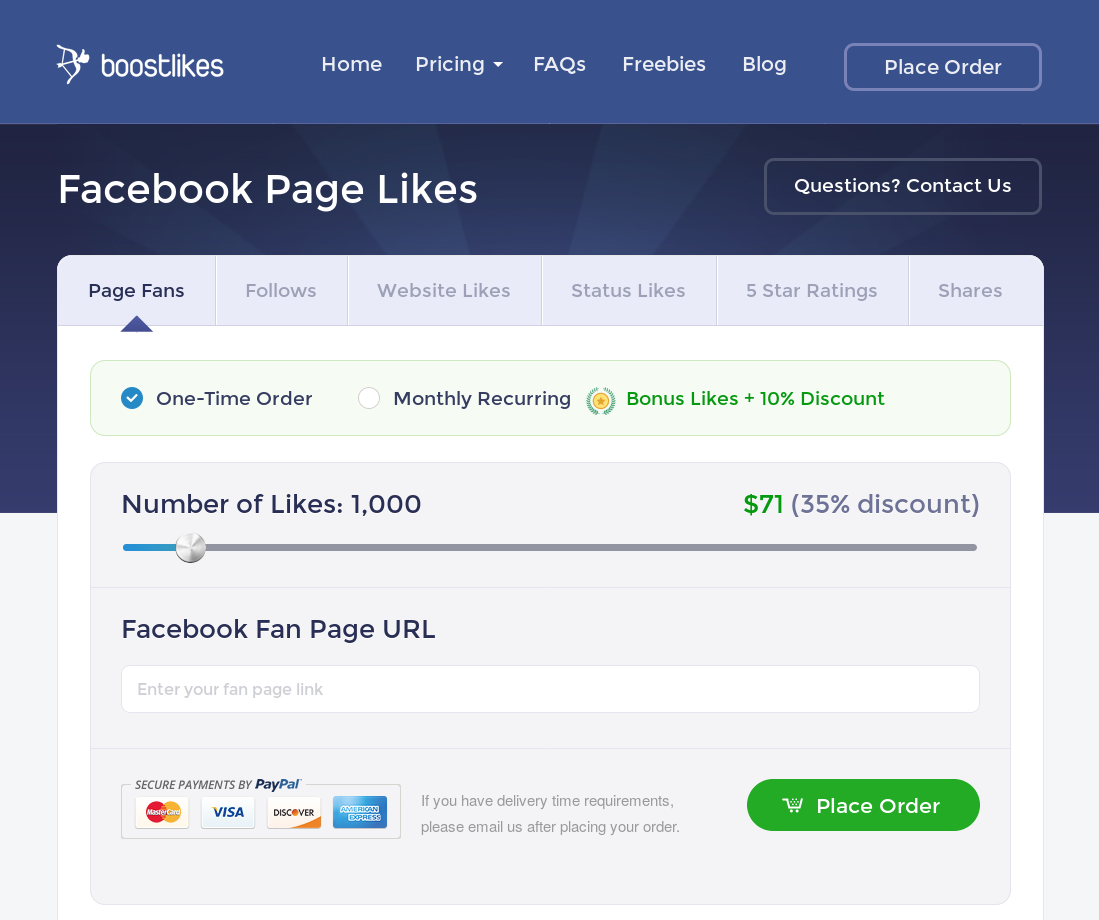
\includegraphics[width=\linewidth]{boostlikes}
  \caption{Screenshot of the Facebook likes service page of boostlikes.com.}
  \label{fig:boostlikes}
\end{figure}

\begin{figure*}
  \centering
  
\includegraphics[width=\textwidth]{socialformulae}
  \caption{Screenshot of the main banner on socialformulae.com.}
  \label{fig:socialformulae}
\end{figure*}

Using Sybils to manipulate public opinion is not only accessible to campaigners
with a large budget. There are marketplaces where anybody can purchase
reputation scores such as Twitter followers. BoostLikes shown on
\autoref{fig:boostlikes} is a professionally presented website, it offers a
large range of services including Facebook likes, Twitter followers, Instagram
followers and YouTube views. SocialFormulae (\autoref{fig:socialformulae}) is a
similar service but at a much lower price point, one thousand Twitter followers
is only \$9.99. There can be little doubt that those companies use automated
bots to provide their services.
% one thousand likes cost \$71 at the time of writing. 

SadBotTrue and its related website Socialpuncher publishes studies on social
media fraud. Two of their studies is particularly useful for demonstrating the
scale of the Sybil attack on Twitter. Firstly, there exist a botnet that consist
of 3 million accounts. Since their creation, they generated 2.6 billion tweets.
Surprisingly, all of the 3 million accounts were created on the same day and the
account names are simply numbered sequentially\cite{sadbottrue}. Such an obvious
activity should be easily detectable by Twitter, but these accounts are still
not closed at the time of writing. Secondly, the top-100 Twitter users have 523
million unique followers between them, but 310 million are bots, that is almost
60\%\cite{socialpuncher}. Suppose the bots all belong to the same attacker, then
they can effectively suppress the opinions of the real users.

Clearly, the defence mechanisms employed by social network and micro-blogging
websites are not adaquate to combat the Sybil attack. If the Sybils infiltrate
even more of our cyberspace, then it may become a form of censorship. In that
case, can we still be considered to have the right to freedom of speech?

TODO Tor
https://blog.torproject.org/blog/tor-security-advisory-relay-early-traffic-confirmation-attack

%%% Local Variables:
%%% mode: latex
%%% TeX-master: "main"
%%% End:
